% Generated by experiments/002-pilot-tiny-ttt/run_null.py + make_figures.py.
\begin{figure}[t]\centering
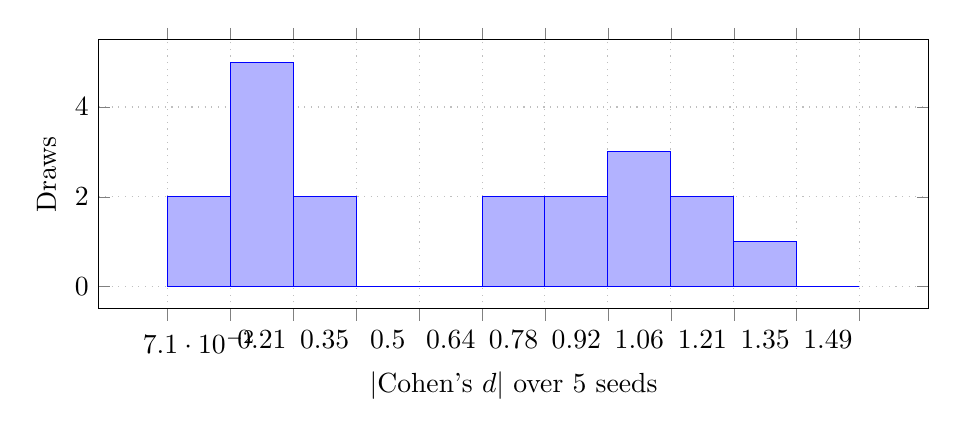
\begin{tikzpicture}
\begin{axis}[width=\columnwidth,height=5cm,ybar interval,
  xlabel={$|$Cohen's $d|$ over 5 seeds},ylabel={Draws},
  grid=both,grid style={dotted}]
\addplot coordinates {(0.071,2) (0.213,5) (0.354,2) (0.496,0) (0.638,0) (0.780,2) (0.921,2) (1.063,3) (1.205,2) (1.347,1) (1.488,0) (1.630,1)};
\end{axis}
\end{tikzpicture}
\caption{Null distribution of the gating effect size. Each of 20 draws compares two benign control streams over five seeds, so the true effect is zero by construction. Median $|d| = 0.816$; 11 of 20 draws clear the pre-registered $d \geq 0.80$ bar with no attacker present, a false-positive rate of 55\%. The deep run's observed $d = 0.831$ sits at the 55th percentile of this null.}
\label{fig:null}
\end{figure}
